\documentclass[12pt]{article}

\usepackage[margin=0.8 in]{geometry}
\usepackage{amsmath}
\usepackage{amssymb}
\usepackage{macros}
\usepackage{mathtools}
\usepackage{enumerate}
\usepackage{verbatim}
\usepackage{amsthm}
\usepackage{hyperref}

\title{Parametrizations of a few curves that show up frequently}
%\content{}



\let \proj \undefined
\renewcommand{\tr}{ \mathrm{tr}}
\DeclareMathOperator{\SU}{SU}
\DeclareMathOperator{\proj}{proj}
\newcommand{\sS}{\mathscr{S}}
\DeclareMathOperator{\comp}{comp}
\newcommand{\A}{\mathcal{A}}
\renewcommand{\D}{\mathcal{D}}
\renewcommand{\e}{\epsilon}
\newcommand{\et}{\tilde{\e}}
\newcommand{\vr}{\mathbf{r}}
\newcommand{\vF}{\mathbf{F}}
\newcommand{\triple}{\iiint_E f(x,y,z)dV}



\newenvironment{solution}
  {\begin{proof}[Solution]}
  {\end{proof}
  
  }
\newtheorem{example}{Example}
\newtheorem{exercise}{Exercise}
\newtheorem{theorem}{Theorem}
\newtheorem{definition}{Definition}


\begin{document}
\maketitle
\begin{itemize}
\item If the curve is part of a circle of radius $r$ and center $(x_0,y_0)$: Use a parametrization of the form $$c(t)=(x_0+r\cos(t),y_0+r\sin(t)), t\in[a,b]$$ for appropriate choices of bounds $a, b$.

\item For an entire ellipse $\frac{x^2}{a^2}+\frac{y^2}{b^2}=1$, you can use $c(t)=(a\cos(t),b\sin(t))$, $t\in[0,2\pi]$. If you have part of it, modify the bounds accordingly.


\begin{figure}
\centering
\parbox{5cm}{
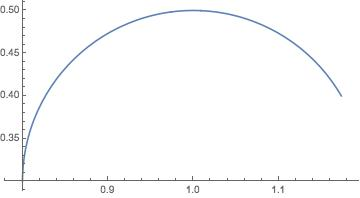
\includegraphics[scale=.3]{circle.jpeg}
\caption{Part of a circle, parametrized as $c(t)=(1+0.2\cos(t),0.3+0.2\sin(t))$, $t\in[\pi/6,\pi]$}
\label{fig1}}
\qquad
\begin{minipage}{5cm}
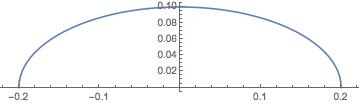
\includegraphics[scale=.3]{ellipse.jpeg}
\caption{Part of an ellipse, parametrized as $c(t)=(0.2\cos(t),0.1\sin(t)),$ $t\in[0,\pi]$.}
\label{fig2}
\end{minipage}
\end{figure}



\item If you have the graph of a function $y=f(x)$, set $x(t)=t$ and $y(t)=f(t)$.

\item If you have a straight line from $(a,b)$ to $(c,d)$, set $x(t)=a+(c-a)t$ and $y(t)=b+(d-b)t$, $t\in [0,1]$.
\item If the curve is more complicated but can be split into simpler parts, write a parametrization for each one of them and write a sum of integrals: if a curve $c$ can be written as the union of two curves $c_1$ and $c_2$, $$\int_c f ds=\int_{c_1}f ds+\int_{c_2} f ds.$$

\begin{figure}[h]
\centering
\parbox{5cm}{
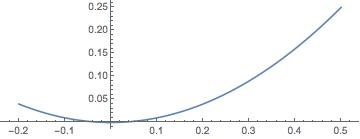
\includegraphics[scale=.2]{graph.jpeg}
\caption{Part of the graph of $f(x)=x^2$, parametrized as $c(t)=(t,t^2)$, $t\in[-0.2,0.5]$.}
\label{fig3}}
\qquad
\begin{minipage}{5cm}
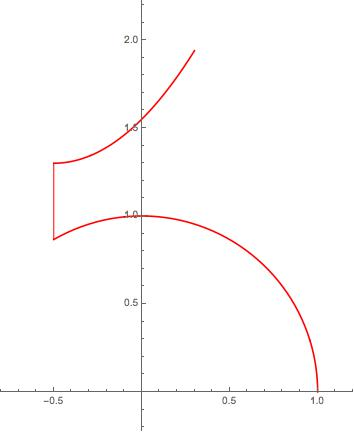
\includegraphics[scale=.3]{pwsm.jpeg}
\caption{A curve consisting of several simpler curves}
\label{fig4}
\end{minipage}
\end{figure}


\item A helix in $\R^3$ about the $z$ axis can be parametrized as $$c(t)=( a\cos(t),b\sin(t), ct),$$ for appropriate bounds on $t$.

\item If you have to parametrize the intersection of two surfaces in $\R^3$, something that can work is to write $c=(x,y,z)$ and use the equations of the surfaces to eliminate two of the variables. Then, set the third one to be $t$. Alternatively, use one equation to eliminate one variable and then once you end up with a something that contains two variables, use one of the above parametrizations of 2 dimensional objects to write them in terms of $t$ (see example in Figure \ref{fig6}).



\end{itemize}
\begin{figure}[h]
\centering
\parbox{5cm}{
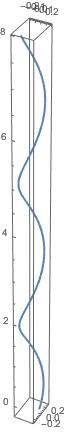
\includegraphics[scale=.3]{helix.jpeg}
\caption{A helix, parametrized as $c(t)=(0.2\cos(t),0.3\sin(t),0.5 t)$, $t\in [-0.2,5\pi]$.}
\label{fig5}}
\qquad
\begin{minipage}{5cm}
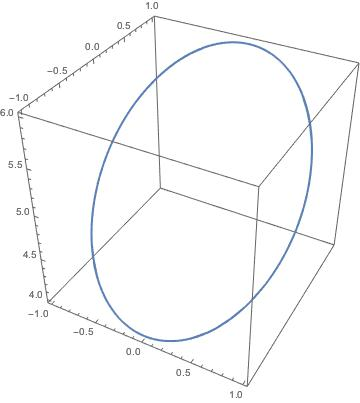
\includegraphics[scale=.3]{intersection.jpeg}
\caption{The intersection of a $x^2+y^2$ and $z=5+y$, parametrized as $c(t)=(\cos(t),\sin(t),5+\sin(t)$, $t\in[0,2\pi]$.}
\label{fig6}
\end{minipage}
\end{figure}



\textbf{General remark:} The definition of the line integral with respect to arc length involves a pretty nasty root expression. This means that for a generic curve its calculation is difficult or impossible. In many cases (and in exams) nice simplifications happen and the integrals can be calculated, so try to be looking for those: in an exam, if the integrals look too complicated you have probably done something wrong in setting them up.


\end{document}

